\section{Problem Statement}
\subsection{Dominant patterns}
\begin{figure}
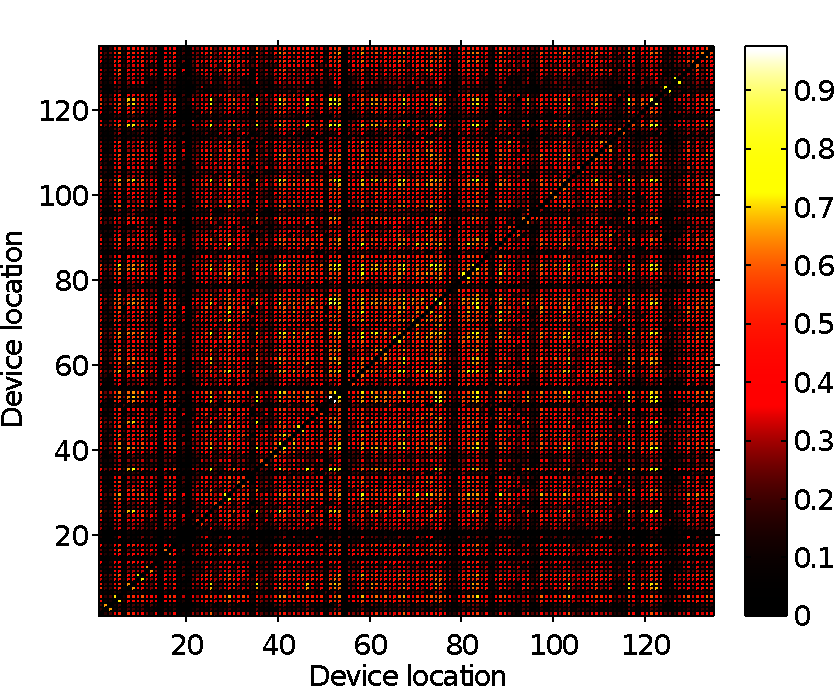
\includegraphics[width=.48\textwidth]{img/heatMap_raw_201106-eps-converted-to.pdf}
\caption{Correlation coefficients of the raw traces from the Engineering Building 2 dataset (Section \ref{data:engbldg2}).
The matrix is ordered such as the devices serving same/adjacent rooms are nearby in the matrix.}
\label{fig:heatmap:raw}
\end{figure}

The first step of the proposed approach is to uncover the devices that are used all together.
The basic tool that allows us to compare the devices power consumption is the correlation coefficient.
However, during our experiments we found that it provides poor help when it is directly applied to the raw signals.
Figure \ref{fig:heatmap:raw} depicts the correlation matrix for 135 devices deployed in the same building (see Section \ref{data:engbldg2} for further information on this dataset).
The devices indexes are selected such as the devices serving the same or adjacent rooms are nearby in the matrix.
We expect devices serving the same room to be used simultaneously thus to feature the highest correlation scores, however, such structure is unseen in the Figure \ref{fig:heatmap:raw}.
In fact the majority of the signals from our dataset are all highly correlated thus this metric prevents us from finding devices that are used in concert.

Thorough inspection of the data reveals that the correlation metric is inefficient with raw signals because all the signals are noisy and contain the same dominant pattern.
For example the two raw signals of Figure \ref{fig:diagram1} are from two independent HVACs serving distinct rooms on different floors.
Although these two devices are independently utilized their signals are highly correlated; namely their correlation coefficient is equal to $0.5675$.
These two 1-week long traces are characterized by the same daily pattern that stands for the common office hours.
This dominant pattern makes the two traces look similar and biases the correlation computation.

\begin{figure}[t!]
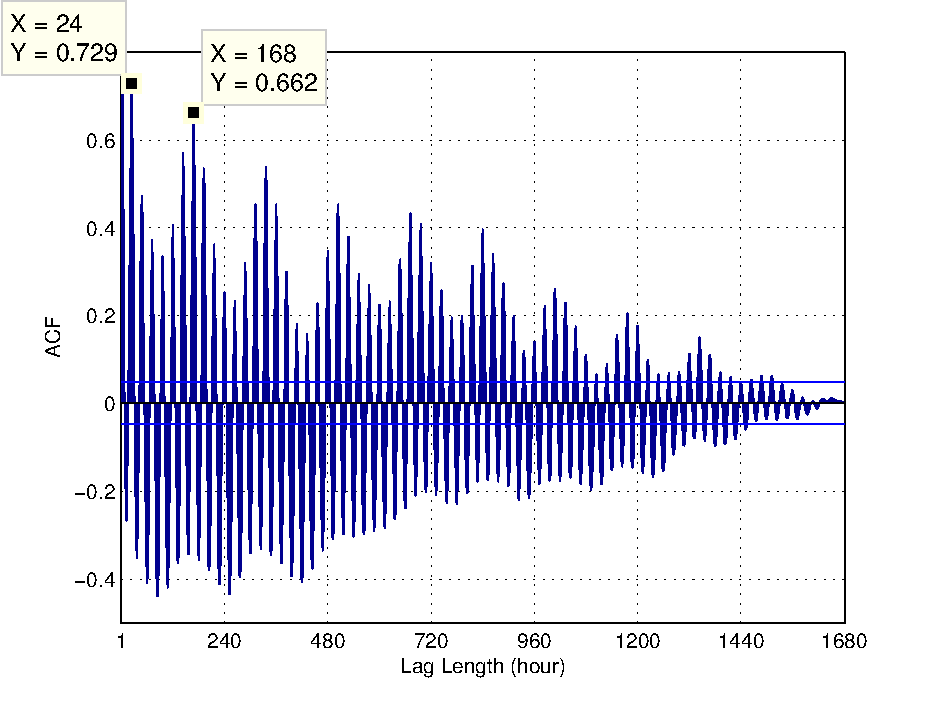
\includegraphics[width=.5\textwidth]{img/acf_101A1_GHP-eps-converted-to.pdf}
\caption{Auto-correlation of a usual signal from the Engineering Building 2 dataset.
The signal features daily and weekly patterns (resp. $x=24$ and $x=168$).}
\label{fig:autocorr}
\end{figure}

Our data inspection uncovered a few dominant patterns that are common to building energy consumption data.
Figure \ref{fig:autocorr} depicts the auto-correlation of a usual electricity consumption signal.
The signal is clearly periodic and contains both daily and weekly patterns.
The weekly pattern stands out due to the distinct power consumption during weekdays and weekends.

One of the major challenge in this work is to discard these patterns and uncover devices intrinsic relationships.
This difficulty is overcome by the proposed intrinsic-correlation estimator presented in Section \ref{methodo:est}.
Then, based on this intrinsic-correlation estimator we propose to monitor over time the devices relationships and detect abnormal device behavior changes that stands for energy wastes (Section \ref{methodo:ano}).
